\chapter{Umsetzung}\label{ch:experiments}

Nach Abschluss der Spezifikation der Benutzeranforderungen wird nun in den dritten Schritt des Human-Centered Design Process übergegangen.
Hier gilt es, dass UX Design zu erstellen, wobei der Style Guide bereits am Ende des letzten Kapitels fertiggestellt wurde.
In den folgenden Abschnitten werden noch die benötigten Interaktionsmöglichkeiten definiert und ein, auf diesen Erkenntnissen aufbauender Prototyp erstellt.

Der Großteil der Anpassungen wird in Form eines Prototypen umgesetzte, um weitere Evaluierungen leichter durchführen zu können und um eventuelle Anpassungen innerhalb kommender Iterationen leichter umsetzen zu können.
Konkret werden die große Anpassungen der Multiselektion und die kleine Änderungen für die Template Properties innerhalb des Prototypen umgesetzte und untersucht, der Filter für die Widget Feature Properties hingegen wird direkt im EB GUIDE Projekt implementiert.
Dies hat den Hintergrund, dass es bei der Multiselektion absehbar ist, dass hier noch einige Anpassungen nötig sein werden, bis das Design und die Funktionalität an die Bedürfnisse der Nutzer angepasst sind.
Das liegt vor allem daran, dass hier noch keinerlei Grundlagen in EB Guide vorhanden sind, auf denen aufgebaut werden kann.
Bei den Template Properties hat die Umsetzung innerhalb des Prototypen den Hintergrund, dass hier nicht sicher gesagt werden kann, ob die Verlagerung der Funktion \glqq publish to template interface\grqq{} von den Nutzern tatsächlich angenommen oder überhaupt an der angedachten Stelle intuitiv erwartet wird.
Es ist hier auch sehr wahrscheinlich, dass an der Darstellung, Positionierung und der Kombination mit der bisherigen Position noch einige Anpassungen stattfinden müssen.
Daher ist es sinnvoll, sich in diesem Fall strikt an den Human-Centered Design Process zu halten und innerhalb dessen Iterationen, solange das UX design zu verbessern bis es sicher den Nutzeranforderungen entspricht.
Ansonsten würde hoher Entwicklungsaufwand in Anpassungen fließen die noch häufig verändert oder komplett verworfen werden müssen.
Die Anpassung des Prototypen kann in diesen Fällen schneller, minimalistischer und mit kleinerem Aufwand erfolgen.

Im Gegensatz dazu macht es Sinn die Filterfunktion direkt in EB Guide zu implementieren.
Aus den bereits durchgeführten Analysen geht hervor, dass dieser Filter einen großen Mehrwert für die Nutzer bieten würde.
Im Gegensatz zu den beiden anderen Änderungen gibt es hier keinen großen Spielraum mehr für Anpassungen, da sich das Design an den bereits bestehenden Filter und Suchfunktionen innerhalb von EB Guide orientiert.
Die einzige eventuelle Anpassung die hier noch auftreten könnte, wäre eine Änderung der Position.
Ob dies jedoch innerhalb eines Prototypen oder im XAML Code stattfindet, macht - betrachtet man den zeitlichen Aufwand - keinen Unterschied.
Daher ist es hier effizienter, die Änderungen direkt zu implementieren und das Verhalten nicht zuerst innerhalb eines Prototypen zu simulieren.

\section {Prototyp Multiselektion und Template Properties}
In den folgenden Abschnitten werden alle relevanten Aspekte im Bezug, auf die im Prototyp umgesetzten Änderungen erläutert.
Zuerst folgt eine kurze Begründung für die Wahl des Prototyping Tools.
Da für diese Arbeit eine Einarbeitung in dieses Tool erfolgt ist, wird dieses darauf folgend in seinen Grundfunktionen erläutert.
Dies ist auch notwendig um die abschließend dargestellte Vorgehensweise zur Erstellung des Prototyps nachvollziehen zu können.
Danach werden die nötigen Interaktionsmöglichkeiten definiert, die dem Nutzer für einen erfolgreichen Umgang mit dem Prototypen simuliert werden müssen, bevor letztlich die Vorgehensweise beschrieben wird um diese Anforderungen umzusetzen.

\subsection {Axure RP}
Axure RP ist eine Software die es ermöglicht Wireframes, Prototypen, Dokumentationen und Spezifikationen für Web-, Mobil- oder Desktopanwendungen zu erstellen.
Dies wird durch Drag and Drop Aktionen, Skalierung und Formatierung von Widgets ermöglicht, mit deren Hilfe man das gewünschte Endprodukt erstellen kann.
Für diese Arbeit ist vor allem die Möglichkeit einen Prototypen zu erstellen wichtig.
Ausschlaggebend für die Wahl dieser Software ist, dass AXURE RP 9 die Möglichkeit bietet dynamische Inhalte zu erstellen und logische Bedingungen in den Prototypen einzubinden.
Da es sich bei EB Guide Studio um ein Modellierungstool handelt, ist ein rein statischer Prototyp nicht ausreichend.
Ebenfalls reicht es nicht aus feste Hotspots zu haben bei deren Klick etwas passiert, sondern es ist notwendig, die in EB Guide herrschenden Einschränkungen für den Nutzer simulieren zu können.

Ein weiterer Grund sich für diese Software zu entscheiden ist es, dass die UX Designer bei Elektrobit ebenfalls mit AXURE RP arbeitet.
So ist zum einen gewährleistet, dass bei den Usabilitytest keine Schwierigkeiten mit der verwendeten Software auftreten würde, zum anderen ist dadurch gleichzeitig ein Ansprechpartner bei auftretenden Problemen vorhanden.

In \cref{fig:Axure_Full} ist das Standardprojekt von AXURE RP zu sehen, welches die Grundlage eines jeden neuen Projektes bildet.

\begin{center}
  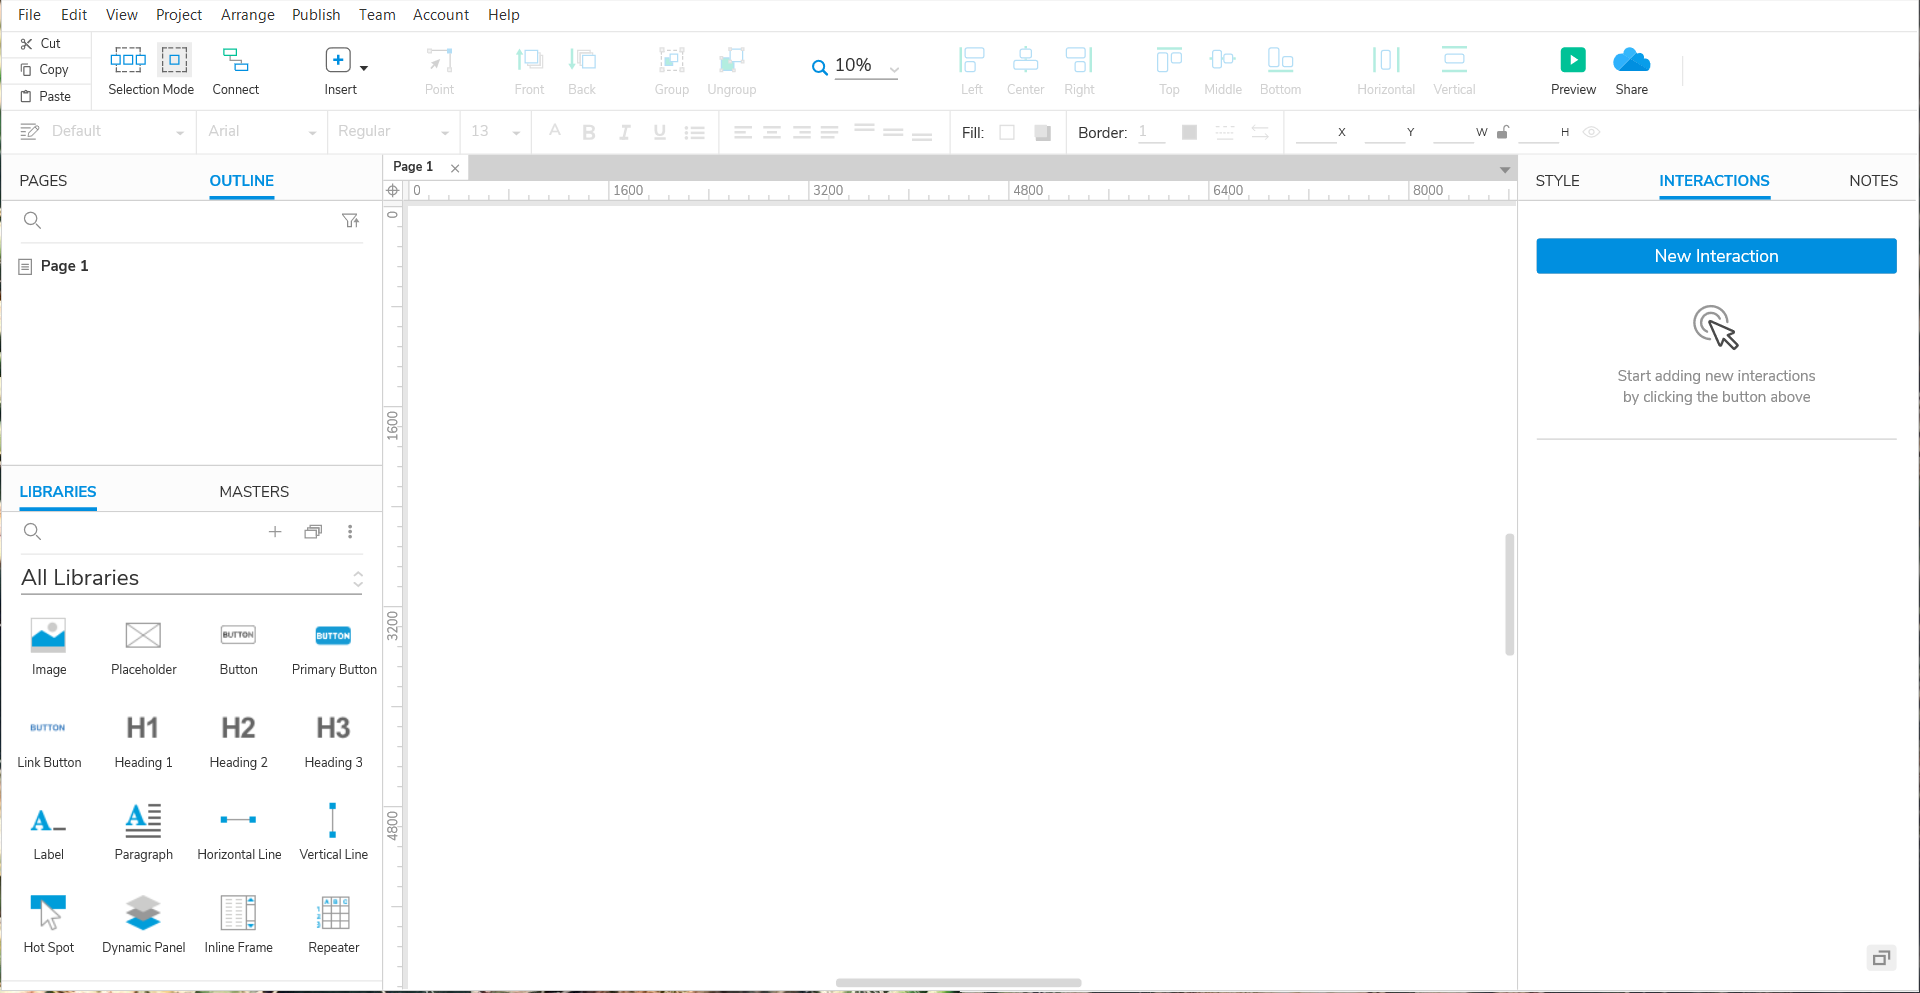
\includegraphics[scale=0.3]{figures/Axure_Full.png}
  \captionof{figure}{Axure RP 9}
  \label{fig:Axure_Full}
\end{center}

In den mittig platzierten Workspace können Elemente aus den Libraries links oder eigene, externe Elemente eingefügt werden.
Zieht man nun beispielsweise eine Droplist und drei Kreiselemente aus den Libraries links in den Workspace, passt sich die Outline wie in \cref{fig:Axure_Outline} zu sehen entsprechend an.
Mithilfe dieser Outline kann man innerhalb des Projektes navigieren, was vor allem praktisch ist wenn sich mehrere Elemente überlagern.
Elemente lassen sich auch zu Dynamic Panels gruppieren, was vor allem dann nötig ist, wenn man ein Drag und Drop Verhalten simulieren möchte, da dies die einzigen Widgets sind die dieses Verhalten unterstützen.

\begin{center}
  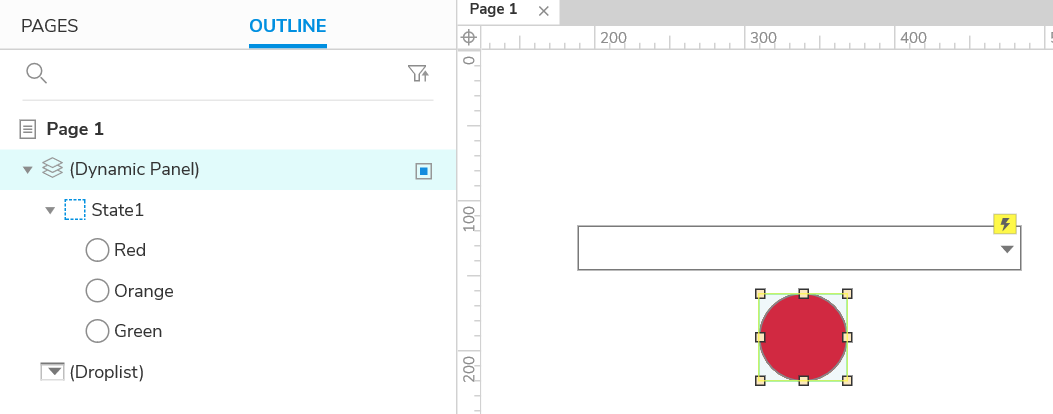
\includegraphics[scale=0.4]{figures/AXURE_Outline.PNG}
  \captionof{figure}{Axure RP 9 Outline}
  \label{fig:Axure_Outline}
\end{center}

Um den drei eingefügten Kreisen unterschiedliche Farben zuzuweisen ist es nötig deren Properties zu bearbeiten.
Dies ist in AXURE RP über das Stlye Panel möglich, welches in \cref{fig:Axure_Style} zu sehen ist.
Hier ist es beispielsweise ebenfalls möglich Skalierungen vorzunehmen oder Umrandungen und Schatten hinzuzufügen.

\begin{center}
  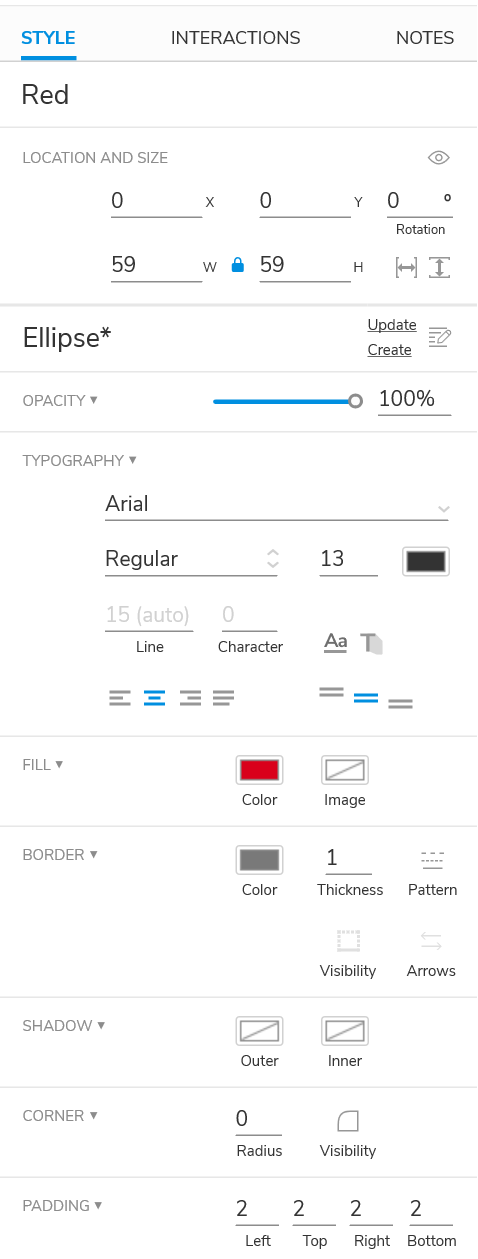
\includegraphics[scale=0.4]{figures/AXURE_Style.PNG}
  \captionof{figure}{Axure RP 9 Style Properties}
  \label{fig:Axure_Style}
\end{center}

Möchte man nun erreichen, dass die Farbe des sichtbaren Kreises sich an der Auswahl innerhalb der Droplist orientiert, muss Logik zu dem Prototypen hinzugefügt werden.
Zuerst ist es, wie in Teil a von \cref{fig:Droplist} zu sehen, nötig Optionen zu der Droplist hinzuzufügen.
Innerhalb des Interactionpanels besteht dann die Möglichkeit, über IF Conditions abzufragen, welche Option aktuell ausgewählt ist.
Passend dazu wir der Kreis mit der gewünschten Farbe angezeigt, und die Visibility der anderen Kreise entsprechend auf null gesetzt.

\begin{figure}%
\centering
\subfloat[][]{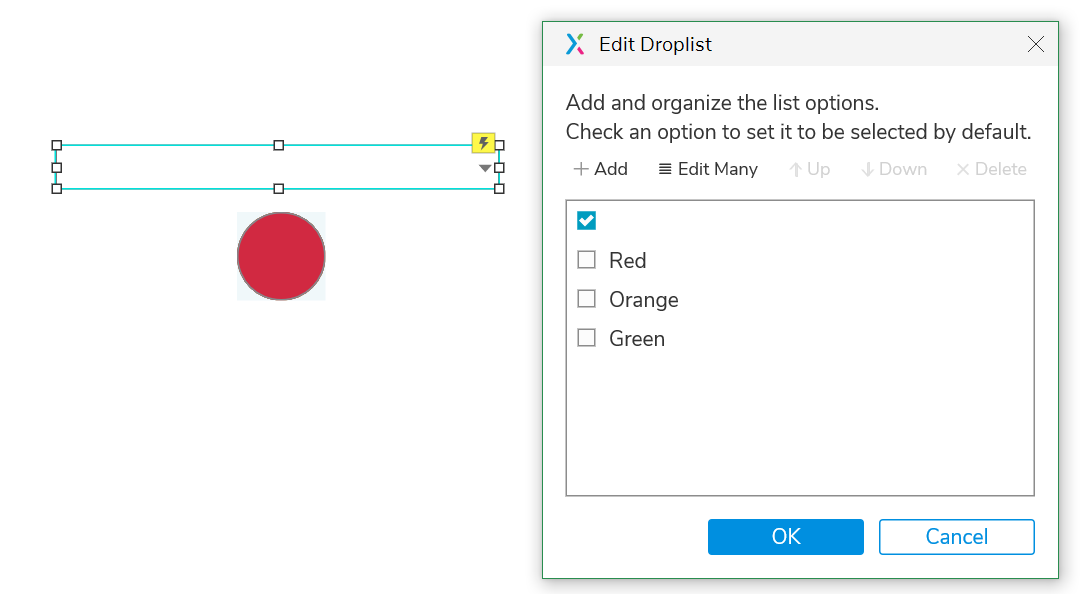
\includegraphics[width=0.5\linewidth]{figures/AXURE_Droplist.PNG}}%
\qquad
\subfloat[][]{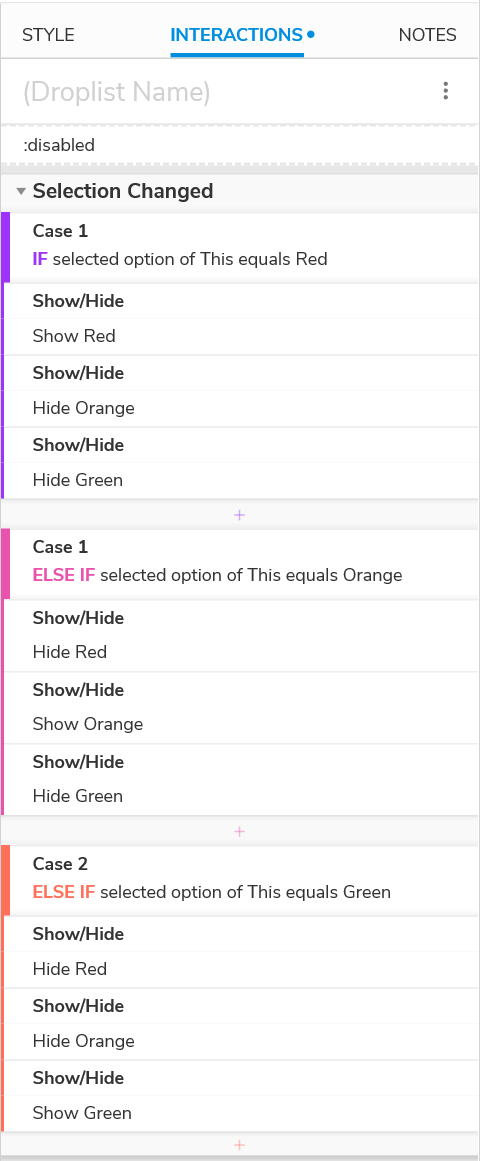
\includegraphics[width=0.3\linewidth]{figures/AXURE_Droplist_Conditions.PNG}}%

\caption{Axure RP Droplist und Conditions}%
\label{fig:Droplist}
\end{figure}

Hat man die Modellierung abgeschlossen, oder möchte Anpassungen überprüfen, bietet AXURE RP die Möglichkeit einer lokalen Preview.
Diese verhält sich exakt so, wie sich der abgeschlossene Prototyp verhalten wird und eignet sich deshalb gut für selbständige Validierung der bisherigen Umsetzung.
Testet man das soeben modellierte Beispiel in der Preview sieht man in \cref{fig:Droplist} , dass sich die Farbe des Kreises, wie gewünscht, immer an die Auswahl der Droplist anpasst.
\begin{figure}%
\centering
\subfloat[][]{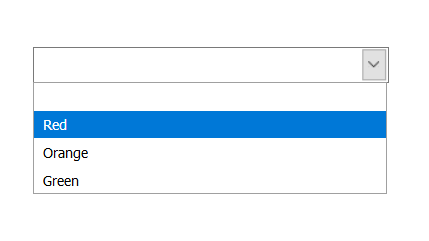
\includegraphics[width=0.3\linewidth]{figures/AXURE_red.PNG}}%
\qquad
\subfloat[][]{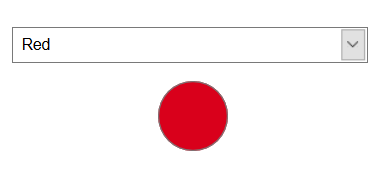
\includegraphics[width=0.3\linewidth]{figures/AXURE_red02.PNG}}%
\qquad
\subfloat[][]{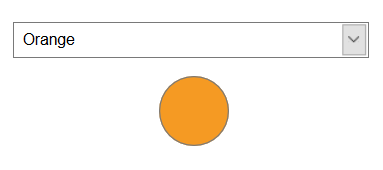
\includegraphics[width=0.3\linewidth]{figures/AXURE_orange.PNG}}%
\qquad
\subfloat[][]{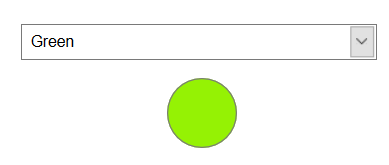
\includegraphics[width=0.3\linewidth]{figures/AXURE_green.PNG}}%

\caption{Axure RP Preview}%
\label{fig:Preview}
\end{figure}

Ist die Modellierung beendet, bietet AXURE RP die Möglichkeit, das Projekt in die AXURE CLOUD zu laden.
Hier können andere Mitarbeiter über einen generierten Link auf das funktionale Endprodukt zugreifen, ohne das eigentliche Projekt sehen oder bearbeiten zu können.
Dadurch ist es nun einerseits möglich andere UX Designer Funktionalitäten des Prototypen testen zu lassen, wobei sie auch an den entsprechenden Stellen Kommentare und TODO's hinterlassen können.
Außerdem besteht durch die Online Verfügbarkeit die Möglichkeit den Prototypen für die Testpersonen im Rahmen des Usability Tests zugänglich zu machen.

\subsection{Interaktionsmöglichkeiten}

Im dritten Schritt des Human-Centered Design Process ist es die Aufgabe des Interaction Designers die Interaktionsmöglichkeiten, die der Prototyp bieten muss, zu spezifizieren.
Dies ist deshalb notwendig, da es gerade bei Prototypen die ein komplexes System simulieren sollen, nicht möglich oder nötig ist alle Funktionen des Systems zu simulieren.
Daher wird vor der Erstellung des Prototyps festgelegt welche Interaktionen von den Nutzern durchführbar sein müssen um die geplanten Verbesserungen validieren zu können.

Für die Prüfung der Usability der Ergänzungen ist es jedoch nicht ausreichend nur die neuen oder ergänzten Funktionen zu simulieren.
Um diese überhaupt anwenden zu können muss der Nutzer einen gewissen Fortschritt innerhalb des Modellierungsprozesses erreicht haben.
Um an diesen Punkt zu gelangen ist es unbedingt notwendig, dass dem Nutzer gewissen Grundfunktionen von EB Guide zur Verfügung stehen.
Das bedeutet für den konkreten Fall dieser Bachelorarbeit, dass es für den Nutzer möglich sein muss wie gewohnt Elemente per Drag and Drop in den View zu ziehen, und diese dort auch frei bewegen zu können.
Ebenfalls müssen die Properties aller Widgets frei anpassbar sein und die Elemente müssen wie gewohnt auf die Eingaben des Nutzers reagieren.
Da sich die Funktion \glqq publish to template interface\grqq{} innerhalb der Templates befindet, muss auch die Möglichkeit bestehen Templates anzulegen.

Darauf aufbauend müssen noch die neuen oder veränderten Funktionen in den Prototypen integriert werden.
Dazu zählt konkret, dass die Funktion \glqq publish to template interface\grqq{} verlagert wird und die vorhandene Möglichkeit dafür vorerst nicht simuliert werden muss.
Zusätzlich muss es nun möglich sein, mehrere Elemente gleichzeitig auszuwählen und hierfür ein Propertiepanel einzublenden.
Die Anpassung der Properties müssen sich in diesem Fall auch auf alle angewählten Elemente auswirken und diese müssen gemeinsam im View bewegt werden können.
Zusätzlich müssen noch die neuen Alignment Actions, sowie die Funktion \glqq Insert in Template\grqq{} angezeigt werden und ausführbar sein.

Da sehr viele unterschiedliche Widget- und Templatetypen in EB Guide existieren, ist es an dieser Stelle des Prozesses auch sinnvoll sich bereits Gedanken über den abschließenden Usability Test zu machen und die Funktionen des Prototypen entsprechend einzuschränken.
Die Modellierer bei Elektrobit setzen hauptsächlich HMIs für den Fahrzeuginnenraum mit EB GUIDE um.
Daher erscheint es sinnvoll für den Usability Test einen minimalistischen Startscreen eines solchen Interfaces modellieren zu lassen.
Da diese, wenn man die Interaktionslogik außen vor lässt, nur aus Images und Labels bestehen ist es ausreichend diese beiden Widgets funktionsfähig zu machen.
Zusätzlich dazu ist es noch notwendig die Menge an verfügbaren Templates einzuschränken.
Für den soeben erläuterten Use Case ist es hier ebenfalls ausreichend nur Image Templates erstellen zu können.
Genauere Erläuterungen zu den Aufgaben innerhalb des Usability Test folgen entsprechend in Kapitel 5.


\subsection{Vorgehensweise}
Im folgenden werden die grundlegenden Vorgehensweisen erläutert die angewandt werden, um den Prototypen zu erstellen.
Es ist im Rahmen dieser Arbeit nicht möglich alle exakten Anpassungen zu erläutern die umgesetzt werden.
Es werden jedoch alle maßgeblichen Konzepte und Funktionen aufgeführt die in Zusammenhang mit den eingebauten Neuerungen stehen.
Alle nicht ausführlich erklärten Änderungen sind auf ähnliche Art und Weise umgesetzt, wie solche die in den nächsten Abschnitten erläutert werden.

\paragraph{Grundlage}
Vor allem bei Expertennutzern ist es wichtig, dass der Prototyp sich nicht nur verhält wie die  gewohnte Software, sondern sich auch optisch an ihr orientiert.
Aus diesem Grund ist der Ansatz zur Modellierung des Prototypen, einen Screenshot der aktuellen Version von EB GUIDE Studio zu machen und diesen als statischen Hintergrund, wie in \cref{fig:Prototyp_01} zu sehen, für das weitere Vorgehen zu verwenden.
Darauf aufbauend können nach und nach Interaktionsmöglichkeiten innerhalb des Prototypen platziert werden.

\begin{center}
  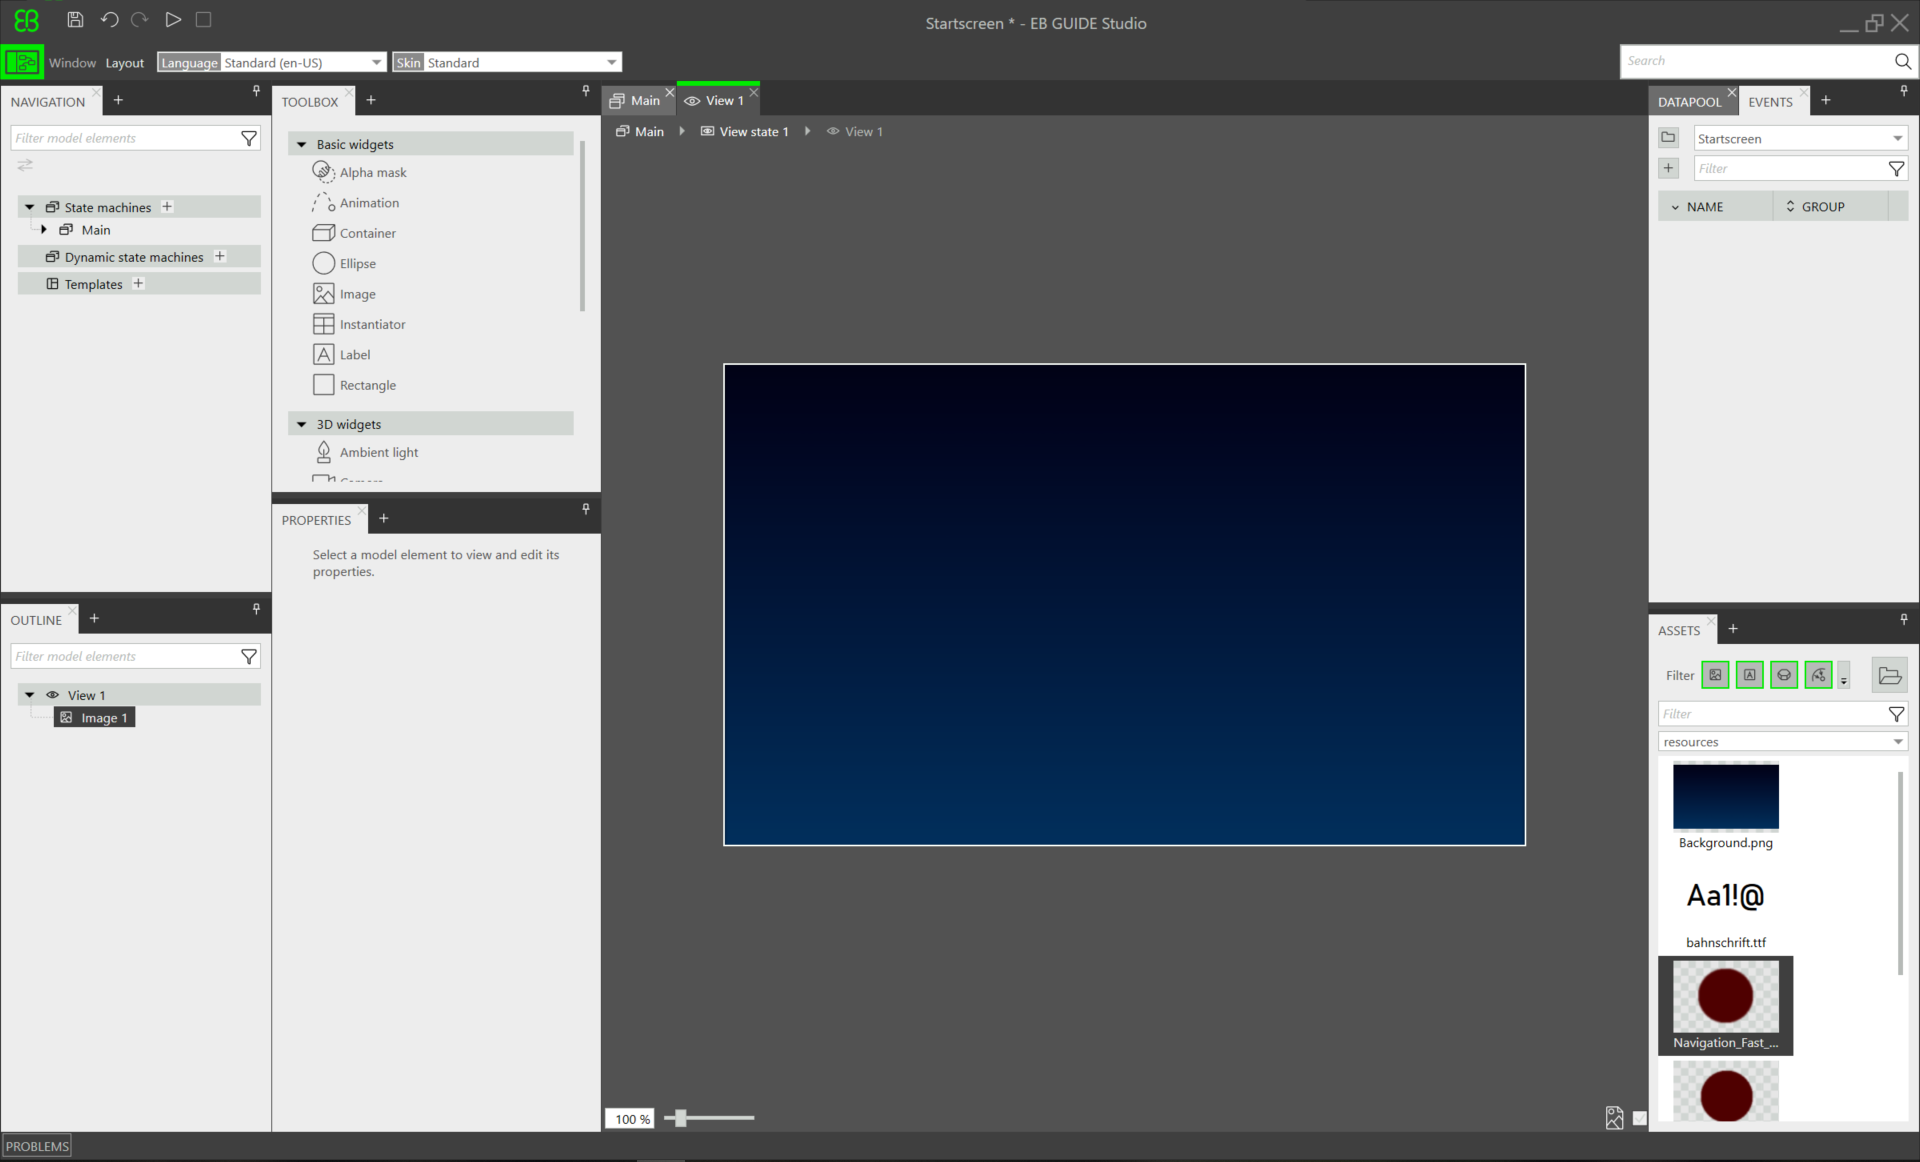
\includegraphics[scale=0.4]{figures/Prototyp_01.PNG}
  \captionof{figure}{Grundlage des Prototyps}
  \label{fig:Prototyp_01}
\end{center}

\paragraph{Assets und Toolbox}
Die Assets und die Toolbox sind wichtige Interaktionsmöglichkeiten für den Nutzer, da von hier alle zur Verfügung stehenden Widgets oder Ressources in den View gezogen werden.
Für beide Elemente wird eine Scrollbar benötigt, da die Nutzer dies an dieser Stelle gewohnt sind, und sonst keine Möglichkeit bestünde alle Widgets und Elemente anzuzeigen.
In AXURE ist es hierfür nötig ein Dynamic Panel zu erstellen und es mit allen benötigten Elementen zu befüllen, die in der Scrollbar vorhanden sein sollen.
Für ein Dynamic Panel ist es möglich eine feste Größe anzulegen, sollten dessen Elemente in der vorgegebenen Dimension nicht alle Platz finden, hat man nun die Möglichkeit Vertikales oder Horizontales Scrolling zu aktivieren.
In \cref{fig:Prototyp_02} sieht man beispielhaft die Umsetzung für das Assetspanel.
Teil a) zeigt die Implementierung mithilfe von ineinander geschachtelter Dynamic Panels, in Teil b) ist das entsprechende Ergebnis im Prototypen zu sehen.

\begin{figure}%
\centering
\subfloat[][]{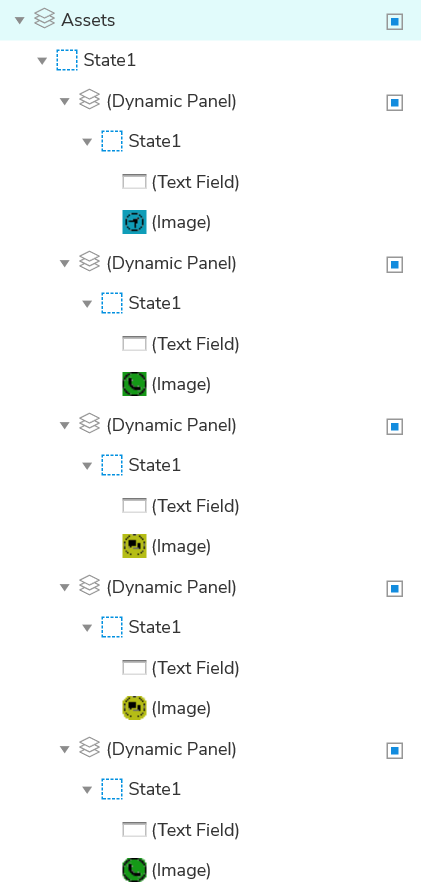
\includegraphics[width=0.4\linewidth]{figures/Prototyp_Assets.PNG}}%
\qquad
\subfloat[][]{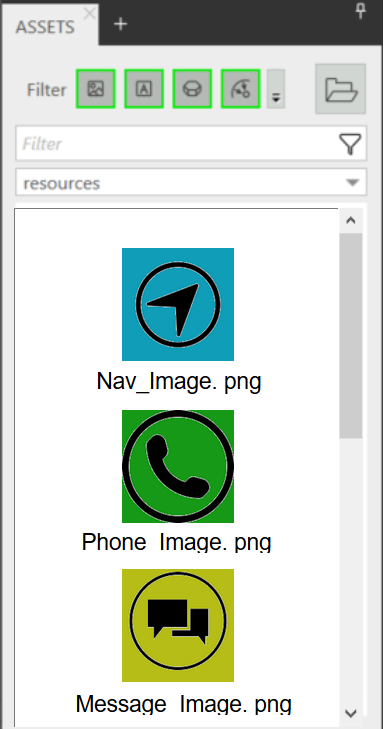
\includegraphics[width=0.4\linewidth]{figures/Prototyp_02.PNG}}%

\caption{Scrollbar für Assets}%
\label{fig:Prototyp_02}
\end{figure}

Der Grund dafür, dass jedes einzelne Bild in den Assets ebenfalls ein Dynamic Panel ist, ist der Tatsache geschuldet, dass dies die einzigen Widgets sind die Drag und Drop unterstützen.
Sie bieten die einzigartigen Interactions \glqq Drag Started\grqq{},\glqq Dragged\grqq{} und \glqq Drag Dropped\grqq{} über welche gesteuert werden kann, wie sich die Items während des Vorgangs verhalten.
Hier erweist es sich als praktisch \glqq Drag Dropped\grqq{} mit einer If Bedingung zu versehen, damit das Element nur über dem dafür vorgesehenen View abgelegt werden kann und nicht zum Beispiel im Bereich der Datapoolitems.

\paragraph{Widget Tree}
Sobald etwas in den View hinzugefügt wird, muss dies für den Nutzer ebenfalls im WidgetTree sichtbar werden.
Dies ist mithilfe eines Screenhots gelöst - zu sehen in \cref{fig:Prototyp_03} -  wobei sich noch weitere Elemente im WidgetTree befinden, die vorläufig überdeckt werden.
Fügt der Nutzer nun das entsprechende Element zum View hinzu, wird die Abdeckung entfernt und das Objekt kann nun über den Widget Tree ausgewählt werden.
Die Interaktionsmöglichkeit wird von AXURE mit den gelben Blitzen gekennzeichnet und ist ebenfalls mit logischen Bedingungen umgesetzt.

\begin{center}
  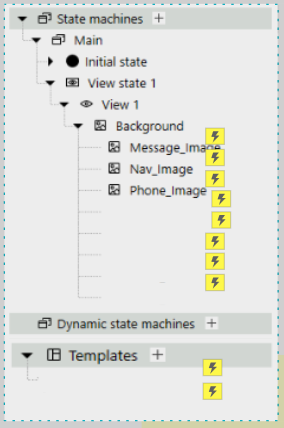
\includegraphics[scale=0.8]{figures/Prototyp_03.PNG}
  \captionof{figure}{Widget Tree}
  \label{fig:Prototyp_03}
\end{center}

\paragraph{Properties}
Um die Interaktion mit allen eingefügten Elementen möglich zu machen, erhält jedes Element sein eigenes Propertiespanel, welches in \cref{fig:Prototyp_04} zu sehen ist.
Damit dem Nutzer immer klar ist, welches Element aktuell ausgewählt ist, wird auch hier das Verhalten von EB GUIDE nachgebaut, indem jedes ausgewählte Element einen grünen Rahmen erhält.
Die Auswahl hierfür muss über das Element selbst oder den Widget Tree möglich sein.

Ist das Objekt aktuell ausgewählt erscheint ein entsprechendes Propertiespanel, welches ebenfalls einen Screenshot beinhaltet der mit Textfeldern überlagert wird.
Diese Felder sind mit globalen Variablen verknüpft, welche wiederum die Properties der Bilder im Workspace von AXURE anpassen.
Dadurch wird es ermöglicht, dass Eingaben in das Textfeld das Objekt verändern und umgekehrt, Bewegungen des Objektes die Werte in den Textfeldern aktualisieren.
Damit wird für den Nutzer das exakt gleiche Verhalten nachmodelliert, welches in EB GUIDE existiert.
Ein identisches Verhalten ist für die Texte modelliert, nur haben diese statt eines Image Properties ein Text Property.

\begin{center}
  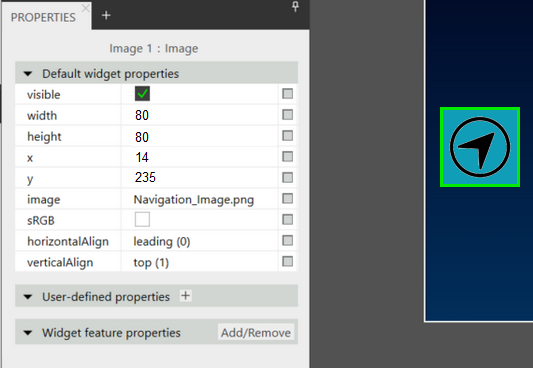
\includegraphics[scale=0.8]{figures/Prototyp_04.PNG}
  \captionof{figure}{Properties Panel}
  \label{fig:Prototyp_04}
\end{center}

\paragraph{Multiselektion}
Ist nur ein Objekt ausgewählt wird der Wert der globalen Variable im entsprechenden Textfeld angezeigt.
Dieser Wert soll bei der Multiselektion jedoch nur angezeigt werden, wenn er für alle ausgewählten Objekte identisch ist.
Da ansonsten ein Strich sichtbar sein soll, ist es hier notwendig die Properties der ausgewählten Objekte zu vergleichen.
Hierfür muss zuerst abgefragt werden welche Objekte ausgewählt sind, um dann deren Properties zu vergleichen.
Da AXURE bei den logischen Bedingungen nur \glqq Match Any\grqq{} oder \glqq Match All\grqq{} unterstützt ist keine Kombination von AND und OR Bedingungen möglich.
Deshalb wird an diesem Punkt nur mit AND Bedingungen in den Abfragen gearbeitet, da jedoch für alle möglichen Kombinationen der drei zur Verfügung stehende Bildern jede Property einzeln abgefragt und angepasst werden muss, ergibt das eine Anzahl von 36 Abfragen.

\begin{center}
  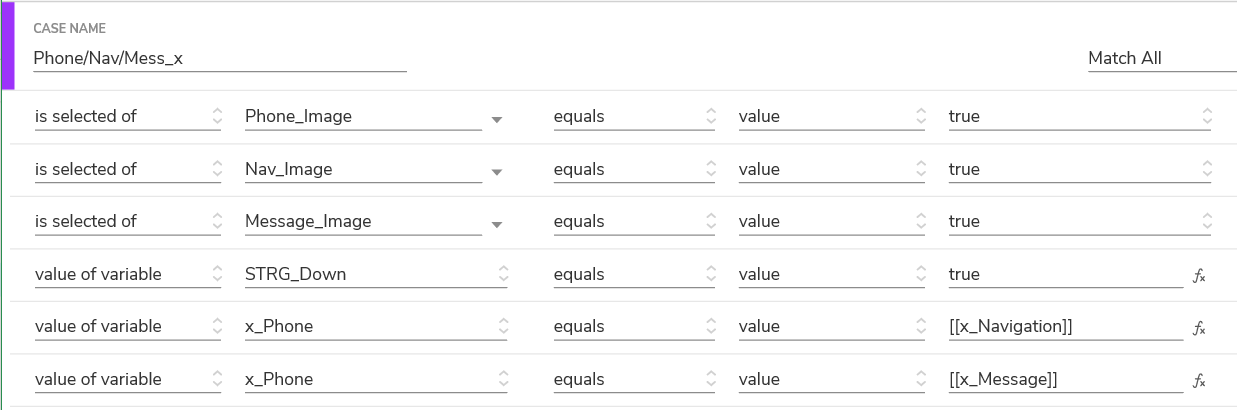
\includegraphics[scale=0.6]{figures/Prototyp_05.PNG}
  \captionof{figure}{Beispielbedingung Multiselektion}
  \label{fig:Prototyp_05}
\end{center}

Auf identische Art und Weise wurde diese Funktionalität für die verfügbaren Labels umgesetzt.
Aufgrund der Performance des Prototyps und der Fehleranfälligkeit wurde auf diese Anpassung bei der gleichzeitigen Auswahl von Texten und Bildern verzichtet.
Es ist hier möglich die Properties anzupassen, es wird jedoch nicht verglichen, ob deren Variablen den gleichen Wert aufweisen, stattdessen wird immer ein Strich angezeigt.
In \cref{fig:Prototyp_05} ist die logische Bedingung für den Fall zu sehen, dass alle drei Bilder gleichzeitig ausgewählt sind und deren x-Koordinate jeweils identisch ist.

Zeitgleich mit den Properties werden bei der Mehrfachselektion die Alignment Actions angezeigt.
Hier wird im Prototypen die Umsetzung in Bezug auf den Testcase eingeschränkt.
Da ein Startscreen modelliert werden soll, reicht die Möglichkeit die Bilder Horizontal aneinander auszurichten, die Vertikale Ausrichtung ist von Texten an Bildern möglich.
In \cref{fig:Prototyp_06} ist die Umsetzung im Prototyp zu sehen, wobei Teil a) bei zwei ausgewählten Bildern und Teil b) bei der gleichzeitigen Auswahl von Bild und Label sichtbar ist.
Die Alignment Actions liegen bei der Auswahl von zwei Objekten des gleichen Typs unten, und bei der Auswahl von zwei unterschiedlichen oben.
Bei letzterem Fall kann eher davon ausgegangen werden. dass keine Properties gemeinsam angepasst werden müssen, sondern die zwei unterschiedlichen Objekte eher aneinander ausgerichtet werden sollen.
Die tatsächliche Ausrichtung wird durch Klick auf den Button ausgelöst, indem der eingegebene Abstand auf den Variablenwert des weiter links oder weiter oben liegenden Objektes aufaddiert wird und der globalen Variable des zweiten Items zugewiesen wird.
Dadurch verschiebt sich das zweite Objekt und der Abstand der zwei Objekte entspricht dem eingegebenem Wert.

\begin{figure}%
\centering
\subfloat[][]{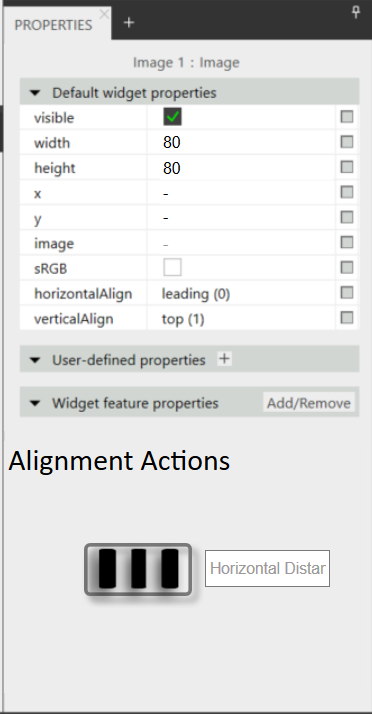
\includegraphics[width=0.3\linewidth]{figures/Prototyp_06.PNG}}%
\qquad
\subfloat[][]{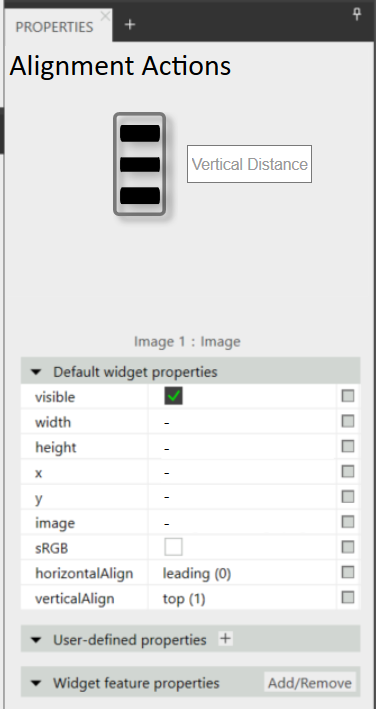
\includegraphics[width=0.3\linewidth]{figures/Prototyp_07.PNG}}%

\caption{Alignment Actions}%
\label{fig:Prototyp_06}
\end{figure}

\paragraph{Templates}
Das Anlegen von Templates wird ebenfalls mit Screenshots simuliert die mit Hotspots versehen werden.
Zusätzlich besteht hier noch die Notwendigkeit einen Imagetab neben dem View anzulegen, da das Erstellen der Templates in einer anderen View stattfindet.
In diesem Tab existiert ebenfalls ein Propertiespanel, die Funktion \glqq publish to template interface\grqq{} geschieht wie geplant über einen Klick auf den Kreis, der sich nach der Auswahl blau einfärbt.
Wird hier ein Wert angepasst wirkt sich das über eine globale Variable auch auf das Template Interface aus.
Eine Änderung im Template Interface darf jedoch nie ein Property des Templates anpassen.
Deshalb wurden hier zwei getrennte Sets von globalen Variablen angelegt, welche nur in eine Richtung synchronisieren.

\begin{center}
  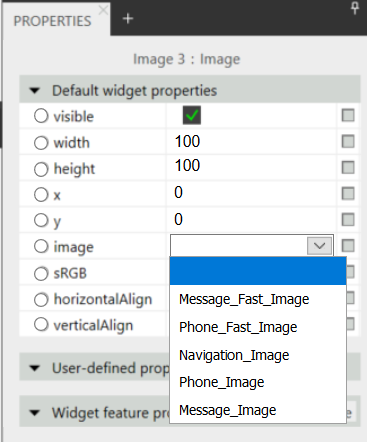
\includegraphics[scale=0.6]{figures/Prototyp_08.PNG}
  \captionof{figure}{Droplist für Images}
  \label{fig:Prototyp_08}
\end{center}

Die Zuweisung der Bilder im Template findet über ein Droplist statt, welche in \cref{fig:Prototyp_08} zu sehen ist.
Die Vorgehensweise, wie der sichtbare Inhalt eines Dynamic Panels mithilfe einer Droplist angepasst werden kann, wurde bereits in Abschnitt 4.1.1 erklärt.
Statt der bunten Kreise befindet sich in diesem Fall jeweils eine Ausführung aller Bilder in den Dynamic Panels welche je nach Auswahl aus der Droplist sichtbar oder unsichtbar geschaltet werden können.
Die alternative Vorgehensweise \glqq Insert in Template\grqq{} funktioniert nach dem selben Prinzip.
Nur wird hier nicht aus der Droplist abgefragt, sondern welches Bild aktuell im Template ausgewählt ist.
Dieses wird dann, nach einem Klick auf den Button entsprechend angezeigt.


\section {Implementierung Filter}
Nach Fertigstellung des Prototyps ist es nun nötig den Filter zu implementieren.
Da hier eine direkte Umsetzung im Sourcecode von EB GUIDE geplant ist, gibt es im Folgenden, nach der Formulierung der Zielsetzung,  einen groben Überblick über den Aufbau des Projektes.
Wie bei der Erstellung des Prototypen im vorherigen Kapitel wird abschließend noch aufgezeigt mit welchem Vorgehen die formulierten Ziele umgesetzt werden.

\subsection {Zielsetzung}
Das Ziel dieses Arbeitsabschnittes ist die Umsetzung des in Abschnitt 3.1.3 definierten optischen und funktionalen Designs.
Da es sich um eine Implementierung handelt ist hier keine Einarbeitung in ein Tool wie AXURE RP notwendig, vielmehr muss der Aufbau des bereits bestehenden Projektes verstanden werden.
Konkret muss für die Umsetzung des Designs eine Filterfunktion implementiert werden, die die bereits vorhandenen Widget Feature Properties nach den Wünschen des Nutzers filtert.
Hierfür wird für den Nutzer eine Eingabemöglichkeit benötigt, mit der er interagieren kann, wie er es von den Filterfunktionen anderer Anwendungen gewohnt ist.
Zusätzlich sollen bei der Nutzereingabe die aktuell bestehenden Kategorien verschwinden und in Echtzeit nur die passenden Features ohne zugehörige Kategorie angezeigt werden.

\subsection {Projektaufbau}

\paragraph{Programmiersprachen und Entwicklungsumgebung}
EB GUIDE Studio wird als WPF Anwendung umgesetzt und ist somit in C\# geschrieben.
WPF ist Teil des .NET-Frameworks 3.0, auf dessen Basis dem Entwickler eine große objektorientierte Klassenbibliothek zur Verfügung steht.
Innerhalb dieser Klassenbibliothek ist auch C\# zu finden, welche eine typsichere, objektorientierte Allzweck-Programmiersprache ist.
Für die Deklaration der Elemente des User Interfaces benutzt WPF die Beschreibungssprache XAML, wleche auf XML basiert.

Da das Projekt firmenintern als eine Visual Studio Solution vorliegt, werden auch sämtliche Implementierungen im Rahmen dieser Arbeit innerhalb dieser Entwicklungsumgebung umgesetzt.

\paragraph{Design Pattern}
In der Projektentwicklung wird das Model-View-ViewModel (MVVM) Design Pattern angewandt.
Bei früheren Entwicklungen von User Interfaces, haben Entwickler häufig eine grafische View erstellt und im Nachhinein die Logik hinzugefügt.
Dies geschieht meist in Form von Eventhandlern, Initialisierungen oder Datenmodellen im Code Behind, was zu einer starken gegenseitigen Abhängigkeit von Interface und der dahinter liegenden Logik führt.
Dadurch entstehen Problematiken wie die Tatsache, dass nicht mehrere Entwickler gleichzeitig an der gleichen View arbeiten können, oder gegenseitig Code unbrauchbar gemacht wird.
Logik und Aussehen eines Interface an einer Stelle zu bündeln führt also zu schlechter Wartbarkeit, Erweiterbarkeit und ist kaum testbar\cite{.g}.
Die aufgeführten Probleme entstehen durch die starke Abhängigkeit der folgenden Komponenten.

\begin{itemize}
 	\item View (User Interface)
 	\item Model (Im User Interface angezeigte Daten)
	\item Zusammenfügender Code (Eventhandling, Abhängigkeiten, Logik)
\end{itemize}

Innerhalb des MVVM Pattern wird dieser zusammenfügende Code als das View Model bezeichnet.
Dessen grundlegende Aufgabe ist es, eine Trennung der View und des Models zu arrangieren und dadurch die Erstellung der Struktur und die Wartung der Anwendung zu vereinfachen.

Sobald sich ein Wert innerhalb des View Models ändert, wir der neue Wert, mithilfe von Data binding und Benachrichtigungen, automatisch im View aktualisiert.
Wenn der Nutzer hingegen mit dem View interagiert, zum Beispiel einen Button drückt, wird eine, sich im View Model befindende Command ausgelöst, die die gewollte Aktion ausführt.
Während dieses Prozesses modifiziert das View Model die Daten des Models, die View selbst führt nie eine direkte Änderung auf dem Model aus.
Tatsächlich weiß die View nicht von der Existenz der Model Klasse, während das Model nicht weiß das die View existiert.

Das Pattern umfasst also die drei Hauptbestandteile:
\begin{itemize}
 	\item View (User Interface)
 	\item Model (Datenzugriffe, Modelklassen)
	\item ViewModel (Vermittler zwischen View und Model)
\end{itemize}

Wie in \cref{fig:MVVM} zu sehen, fungiert das ViewModel als Schnittstelle zwischen dem Model und der View. Es stellt ein Data binding zwischen den beiden Instanzen bereit und verarbeitet über Commands alle Eingaben des Nutzers.
Die View bindet ihre Kontrollwerte an Properties des ViewModels, welche im Gegenzug die Daten der Modelobjekte bereit stellen.

\begin{center}
  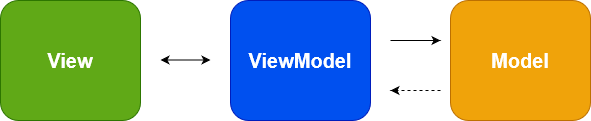
\includegraphics[scale=0.6]{figures/MVVM.PNG}
  \captionof{figure}{Model-View-ViewModel (MVVM) Design Pattern}
  \label{fig:MVVM}
\end{center}

Im aktuellen Projekt werden alle benötigten Models, meist in Form von Interfaces, in die ViewModel Klasse WidgetFeaturesOverlayViewModel importiert.
Aufgrund des Datenschutzes ist es nicht möglich, die genauen Models und die vollständige Implementierung der Klassen in dieser Arbeit offenzulegen.
Die in den folgenden Kapiteln erläuterten Ergänzungen, werden in die soeben erwähnte ViewMode Klassen und der dazugehörigen View WidgetFeaturesOverlayViewModel.xaml eingearbeitet.

\paragraph{CollectionViewSource}
Die zu filternden Elemente liegen innerhalb des Projektes bereits in Form einer CollectionViewSource vor.
Diese besitzt die Eigenschaften View und Source, welche jeweils unterschiedliche Varianten einer Collection beinhalten können.
Die View kann man hier als eine, über der Source liegenden Ebene verstehen, mit deren Hilfe die Darstellung der Collection manipuliert werden kann.
Das geschieht beispielsweise durch sortieren, filtern und gruppieren von Elementen, ohne jedoch die darunter liegende Source an sich zu verändern.
Falls die Source das Interface INotifyCollectionChanged implementiert, werden alle Änderungen, die durch das CollectionChanged event entstehen, an die View weitergeleitet.\cite{dotnetbot.}

Im konkreten Fall des vorliegenden Projektes besteht die Source aus einer ObservableCollection, welche die Feature Models des aktuell ausgewählten Widgets beinhaltet.
Eine ObservableCollection ist eine Collection dynamischer Daten, welche Benachrichtigungen für das Hinzufügen, Entfernen, oder Neuladen der Liste bereit stellt.
\cite{dotnetbot.c}
Aktuell wird die CollectionViewSource gruppiert und sortiert, wodurch die Einteilung in Kategorien und die alphabetische Sortierung in der View erzeugt wird.

\subsection {Vorgehensweise}
Zusätzlich zur Gruppierung und Sortierung stellt die CollectionViewSource ein Filter Event bereit.
Diese Filter können mithilfe der View auf die Collection angewendet werden. 
Das bedeutet konkret, dass ein Item zwar in der Collection Source existiert, mithilfe des Filterevents jedoch nur ein ausgewählter Teil dieser Collection in der View angezeigt wird.\cite{dotnetbot.b}
Das Event kann durch Setzen eines EventHandlers genutzt werden, welcher die gewünschte Filterlogik bereitstellen kann.
Dieser Eventhandler ist in Auflistung \ref{lst:CollectionViewSource}, in den Zeilen 22 bis 23 zu sehen, die dazugehörige Filterlogik in Auflistung \ref{lst:Filter}.

\newpage
\lstinputlisting[caption={CollectionViewSource()},captionpos=b, label=lst:CollectionViewSource]{listings/ICollectionView.cs}

Innerhalb der Filterfunktion muss zuerst abgefragt werden, ob der Filtertext leer ist oder Text beinhaltet.
Falls dies der Fall ist, ist es nicht nötig die Features zu filtern, weshalb alle verfügbaren mithilfe von Accepted zurückgegeben werden.
Sollte der Filtertext jedoch initialisiert worden sein, wird jedes Item innerhalb des Events als FeatureViewModel gespeichert.
FeatureViewModels enthalten alle relevanten Informationen über die Features.
Dazu zählt auch deren Namen, weshalb an dieser Stelle überprüft werden kann, ob die Eingabe des Nutzers einem Featurenamen entspricht oder in diesem enthalten ist.
Sollte dies der Fall sein, wird das Feature der gefilterten View hinzugefügt, anderenfalls wird das Feature durch den Filter entfernt.

\lstinputlisting[caption={Widget Properties Filter},captionpos=b,  label=lst:Filter]{listings/Filter.cs}

Die Grundstruktur des in Auflistung \ref{lst:CollectionViewSource} zu sehenden ICollectionView war im Projekt bereits vorhanden. 
Zusätzlich zu dem eben erwähnten Filter ist noch die If Abfrage in Zeile 9 ergänzt worden.
Diese dient dazu die ausklappbaren Kategorien auszublenden, sobald ein Filterbegriff eingegeben wird.
Die zweite Bedingung der If Abfrage in den Zeilen 5 und 6 ist ebenfalls neu hinzugefügt worden, um die Filterung in Echtzeit zu ermöglichen.
Bis jetzt war der erste Teil der Abfrage ausreichend, da die Liste nur einmal bei der Anzeige des entsprechenden Panels aktualisiert und angelegt werden musste, nach der Implementierung der Filterfunktion ist dies jedoch bei jeder Änderung des Filterbegriffes notwendig.
Aus diesem Grund wird nun auch abgefragt ob der Filtertext aktuell Text enthält, damit bei jedem ChangeEvent die Liste neu gefiltert wird.

Ausgelöst wird dieses ChangeEvent über den in Auflistung \ref{lst:Properties} zu sehenden Setter des Filtertextes.
Sobald eine Änderung im Textfeld registriert wird, schickt die View ein Update an das ViewModel, wodurch der Filtertext angepasst wird.
Zusätzlich dazu wird dem AvailableWidgetFeatures in Auflistung \ref{lst:CollectionViewSource} über das OnPropertyChanged Event mitgeteilt, dass die View aktualisiert werden muss.


\lstinputlisting[caption={Filtertext Properties},captionpos=b,  label=lst:Properties]{listings/Filter_Properties.cs}

Das Update vonseiten der View wird aufgrund des, in Auflistung \ref{lst:XAML} in Zeile 5 bis 6 zu sehenden, UpdateSourceTriggers ausgelöst. 
Hier wird über die Angabe des Paths festgelegt, dass bei jeder Änderung der TextProperty die Properties des FilterTextes aktualisiert werden.
Zusätzlich wird hier ein Delay von 100 eingeführt, um die Filterung in Echtzeit zu ermöglichen.
Dieses Zeitintervall führt dazu, dass der Nutzer auch bei einer schnellen Eingabe nicht durch eine verzögerte Aktualisierung in seinem Arbeitsablauf unterbrochen  oder verlangsamt wird.

\lstinputlisting[caption={Filterpanel in xaml},captionpos=b,  label=lst:XAML]{listings/Filter_Panel.xaml}


